
%%%%%%%%%%%%%%%%%%%%%%% file typeinst.tex %%%%%%%%%%%%%%%%%%%%%%%%%
%
% This is the LaTeX source for the instructions to authors using
% the LaTeX document class 'llncs.cls' for contributions to
% the Lecture Notes in Computer Sciences series.
% http://www.springer.com/lncs       Springer Heidelberg 2006/05/04
%
% It may be used as a template for your own input - copy it
% to a new file with a new name and use it as the basis
% for your article.
%
% NB: the document class 'llncs' has its own and detailed documentation, see
% ftp://ftp.springer.de/data/pubftp/pub/tex/latex/llncs/latex2e/llncsdoc.pdf
%
%%%%%%%%%%%%%%%%%%%%%%%%%%%%%%%%%%%%%%%%%%%%%%%%%%%%%%%%%%%%%%%%%%%


\documentclass[runningheads,a4paper]{llncs}

\usepackage{amssymb}
\setcounter{tocdepth}{3}
\usepackage{graphicx}
\usepackage{float}
\usepackage[full]{complexity}
\usepackage{amsmath}
%\usepackage{amsfonts}
%\usepackage{amsthm}
\usepackage{subfigure}
%\usepackage{caption}
%\usepackage{subcaption}
%\usepackage{cite}
\usepackage{hyperref}
\usepackage{url}
\usepackage{clrscode4e}
\usepackage{verbatim}
\urlstyle{same}
\newcommand{\keywords}[1]{\par\addvspace\baselineskip
\noindent\keywordname\enspace\ignorespaces#1}

% Uniform numbering for previously defined theorem environments (e.g., LNCS).
\makeatletter
\let\c@lemma=\c@theorem
\let\c@corollary=\c@theorem
\let\c@fact=\c@theorem
\makeatother

% Redefinition of LNCS or SODA or Springer proof environment to put a \Box at
% the end of every proof.
\let\realendproof=\endproof
\def\endproof{\hspace*{\fill}$\Box$\realendproof}

\begin{document}

\mainmatter  % start of an individual contribution

% first the title is needed
\title{The Complexity of Determining Critical Sets}

% a short form should be given in case it is too long for the running head
\titlerunning{The Complexity of Determining Critical Sets}

% the name(s) of the author(s) follow(s) next
%
% NB: Chinese authors should write their first names(s) in front of
% their surnames. This ensures that the names appear correctly in
% the running heads and the author index.
%
\author{Fermi Ma \and Ariel Schvartzman \and Erik Waingarten}
%
\authorrunning{Fermi Ma \and Ariel Schvartzman \and Erik Waingarten}
% (feature abused for this document to repeat the title also on left hand pages)

% the affiliations are given next; don't give your e-mail address
% unless you accept that it will be published
\institute{MIT,\\
77 Mass Ave., Cambridge, MA 02139, USA, \\
\protect\url{{fermima,arielsc,eaw}@mit.edu}}

%
% NB: a more complex sample for affiliations and the mapping to the
% corresponding authors can be found in the file "llncs.dem"
% (search for the string "\mainmatter" where a contribution starts).
% "llncs.dem" accompanies the document class "llncs.cls".
%

\maketitle

\subsection{Triangle Partition}\label{S:TP}

The Triangle Partition problem is the following:
\begin{quote}
\textbf{Instance}: An undirected graph $G = (V, E)$.\\
\textbf{Question}: Can we partition $E$ into disjoint triangles?
\end{quote}

Holyer \cite{holyer1981np} showed this problem is $\NP$-complete. His main tool (shown in Figure~\ref{fig:holyergraph}) was the graph $H_{3, p}$, which has only two possible triangle partitions. Note this is a small section of the graph, and it continues with these type of tilings.
\begin{figure}
\label{fig:holyergraph}
\centering
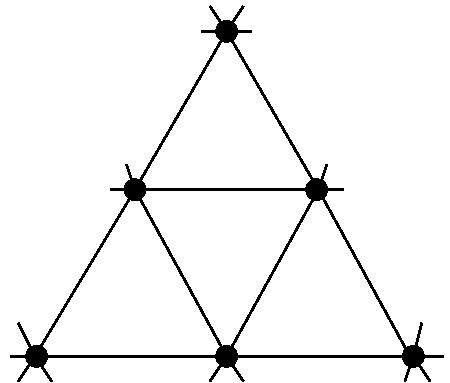
\includegraphics[width=0.4\linewidth]{Holyergraph.pdf}
\caption{Holyer's $H_{3,p}$ graph}
\end{figure}

The $\mathsf{FCP}$ version of the problem is to find the fewest number of triangles we must give in order for there to be a unique triangle partition. For example, in $H_{3,p}$ (Figure~\ref{fig:holyergraph}), once you specify one triangle in the partition, there is only one way to partition the graph in accordance with that triangle.

We claim $\mathsf{FCP}$ Triangle Partition is $\Sigma_2^P$-complete. We give a quick summary of Holyer's reduction which highlights the ideas we will use to show it is $\Sigma_2^P$-complete. 

\subsubsection{Holyer's Reduction for Triangle Partition}
Holyer uses the graph $H_{3,p}$ (shown in Figure~\ref{fig:holyergraph}) to represent variables and literals. Each graph can only be partitioned in one of two ways. One way will correspond to a true setting, the other will correspond to a false setting. They called the two possible partitions the $T$-partition and the $F$-partition. We will refer to a $T$-partition when the individual triangles are pointing down, and $F$-partition when individual triangles are pointing up (see Figures~\ref{fig:tpart} and \ref{fig:fpart}).

\begin{figure}
\begin{minipage}{0.5\linewidth}
\centering
\includegraphics[scale=0.5]{Tpartition.pdf}
\label{fig:tpart}
\caption{$H_{3,p}$ partitioned like a $T$-partition. In a particular part of the graph, one triangle 'pointing down' specified.}
\end{minipage}
\hfill
\begin{minipage}{0.5\linewidth}
\centering
\label{fig:fpart}
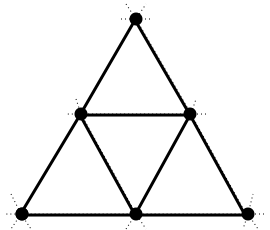
\includegraphics[scale=0.5]{Fpartition.pdf}
\caption{$H_{3,p}$ partitioned like an $F$-partition. In a particular part of the graph, three triangles 'pointing up' specified.}
\end{minipage}
\end{figure}

The authors also use the graphs to make clauses. They show a way to join three $H_{3,p}$ graphs such that exactly one of them will be $F$-partitioned. The three graphs will correspond to literals in the clause. Then they give a way to combine the literals with the variables such that if a literal is set to an $F$-partition, the corresponding variable must be set to either a $T$-partition (in the case where the literal is positive), or an $F$-partition (if the literal is negative). However, if the literal is a $T$-partition, then it does not matter what the variable is set to. 

In particular, there are three important properties of Holyer's reduction which we utilize:
\begin{enumerate}
\item We have variable and literal gadgets. These are graphs which can be partitioned in two possible ways. A graph is $T$-partitioned if it corresponds to setting that variable to true and $F$-partitioned otherwise.  
\item A clause gadget is a join between three literal gadgets. The clause gadget has a triangle partition if exactly one of the literals is $F$-partitioned.
\item A literal is joined with a variable. If the literal is $F$-partitioned, then there are two options:
\begin{itemize}
\item If the literal is the positive variable, then the variable must be $T$-partitioned.
\item If the literal is the negative variable, then the variable must be $F$-partitioned.
\end{itemize}
\end{enumerate}

If there exists a triangle partition of the graph, then each clause is satisfied by at least one literal. That literal gadget will be $F$-partitioned and it will cause the variable to take a particular partition, giving it its assignment. 

We describe gadgets needed to join the reduction. The first will be the gadget for joining literals into a clause. The one property we want is that the joined graphs can be partitioned into triangles if and only if exactly one of the literals is $F$-partitioned. 

We will imagine the three literal graphs stacked up, and we will join them at 6 vertices. Then we will remove the inner edges. Figure~\ref{fig:join3} shows the gadget. The edges of the gadget shown must be partitioned into some triangle. This will be an upward facing triangle with some edges from the literal graph. Note that by joining an upwards facing triangle, we can require exactly one of the literal graphs to be $T$-partitioned instead of $F$-partitioned. For notational purposes, we will denote these kinds of joins by dashed lines.

\begin{figure}
\label{fig:join3}
\centering
\includegraphics[width=0.4\linewidth]{Holyer_join_3.pdf}
\caption{Holyer's clause gadget. Three literal graphs are joined so that exactly one must be $F$-partitioned.}
\end{figure} 

The gadget to join two graphs is simpler. Again, we think of two graphs as stacked and then we join one upward facing triangle. Figure~\ref{fig:join2} shows how two graphs may come together. Note that both graphs cannot be $F$-partitioned. If both graphs wanted to be $F$-partitioned, both would need to utilize the upward facing triangle shown in Figure~\ref{fig:join2}. So there are two possibilities: either one graph is $F$-partitioned and the other is $T$-partitioned, or they are both $T$-partition. We will show these kinds of joins by arrows between graphs. Note that there is some ambiguity in the notation with the arrows. If a literal has an arrow pointing to a variable, then if the literal is $F$-partition, then it makes the variable $T$-partitioned (if the variable appears positive in the literal), or $F$-partitioned (if the variable appears negative in the literal).

\begin{figure}
\label{fig:join2}
\centering
\includegraphics[width=0.2\linewidth]{Holyer_join_2.pdf}
\end{figure}

Similar to before, we can instead join a downward facing triangle and require that graphs joined are not both $T$-partitioned. 

\begin{figure}
\label{fig:holyeroverview}
\centering
\includegraphics[width=\linewidth]{Holyer_reduction.pdf}
\caption{Triangle partition instance corresponding to the formula $\phi = (x \vee y \vee z) \wedge (\overline{x} \vee z \vee \overline{w}) \wedge (y \vee z \vee w)$. The white circles correspond to $H_{3,p}$ graphs. Dashed lines correspond to three-way joins and arrows correspond to two way joins.}
\end{figure}

\subsubsection{$\mathsf{FCP}$ Triangle Partition} 

There is one small issue with Holyer's reduction if we try to apply a General Clue Reduction. The issue lies in the fact that even if we partition all the variables corresponding to their assignments, if there are clauses with multiple true literals, there is ambiguity in how to partition the triangles in the clause gadgets. This might encourage the Triangle Partition algorithm to seek triangle partitions which correspond to satisfying assignments which maximize the number of clauses with only one true literal. In doing so, we might not be minimizing the number of clues for $\phi$.

In order to fix this issue, we will introduce some additional ambiguity for exactly the cases when there are clauses with only one true variable. We will define a mapping $f$ from $3\SAT$ instances to Triangle Partition instances. The map will be a reduction similar to Holyer's reduction. Then we will show that the minimum clues of $3\SAT$ and Triangle Partition can be related. 

\subsubsection{Reduction} Similar to Hoyler's reduction, we use $H_{3,p}$ graphs. We will join them using the three-way joins and the two-way joins described in Figure~\ref{fig:join3} and \ref{fig:join2}. For notational purposes, we again use the fact that white circles correspond to $H_{3,p}$ graphs, dashed lines between three white circles correspond to a three-way join, and arrows correspond to two-way joins.

We give the clause gadget in Figure~\ref{fig:clausegadget}. Note that each clause connects the literals to the variables as in Holyer's reduction, but we add some extra graphs. The important added graphs are labeled $1, 2,$ and 3. 
\begin{figure}
\label{fig:clausegadget}
\centering
\includegraphics[width=\linewidth]{Triangle_clause_gadget.pdf}
\caption{The clause gadget connecting corresponding to variables $x, y$ and $z$. The dashed lines correspond to three-way joins, and the arrows correspond to two way joins. The arrow between $l_x$ and $x$ indicates that if $l_x$ is $F$-partitioned, then $x$ is partitioned corresponding to the assignment that makes $l_x$ true. The arrow from $l_x$ to $2$ corresponds to the join where if $l_x$ is $F$-partitioned, then $2$ is $T$-partitioned. The arrow from $x$ to $2$ indicates that if $x$ is partitioned according to the assignment that makes $l_x$ true, then $2$ is $T$-partitioned.}
\end{figure}


\begin{theorem}
$\mathsf{FCP}$ Triangle Partition is $\Sigma_2^P$-complete.
\end{theorem}

\begin{proof}
We reduce from $3\SAT$. We will give a mapping $f$ from instances of $3\SAT$ to instances of Triangle Partition. Let $M_{3\SAT}(\phi)$ be the minimum number of assigned variables needed for $\phi$ to have a unique satisfying assignment. Likewise, $M_{T}(f(\phi))$ be the minimum number of triangles specified so that there is a unique triangle partition with these triangles as parts of the partition. We will show
\[ M_{T}(f(\phi)) = M_{3\SAT}(\phi) + m \]
Where $m$ is the number of clauses in $\phi$. This will show that Triangle Partition is $\Sigma_2^P$-complete.
\end{proof}

\begin{lemma}
Let $\phi$ be a Boolean formula and $M_{3\SAT}(\phi)$ be the minimum number of assignments needed so that the remaining formula is uniquely satisfiable. Also, suppose $\phi$ contains $m$ clauses. Then
\[ M_T(f(\phi)) = M_{3\SAT}(\phi) + m \]
\end{lemma}

\begin{proof}
First, we show $M_T(f(\phi)) \leq M_{3\SAT}(\phi) + m$. Suppose $c_\phi$ was a set of assignments for $\phi$ with the remaining formula having a unique satisfying assignment. Suppose this unique satisfying assignment is $S$. We give a set $c_{f(\phi)}$ of $|c_\phi| + m$ triangles which uniquely specify a triangle partition. 

First, if $x$ contains an assignment in $c_\phi$, then we include a triangle from the $H_{3,p}$ graph corresponding to $x$. If $x$ is set to true, we make $x$ a $T$-partition. If $x$ is set to false, we make it an $F$-partition. We include this triangle in $c_{f(x)}$. 

By assumption that $S$ is a satisfying assignment, each clause $C$ will have at least one true literal. So for each $C$:
\begin{itemize}
\item Suppose $C$ has exactly one true literal. Lets suppose this literal is $l_y$ (looking at Figure~\ref{fig:clausegadget}). So $l_y$ is necessarily $F$-partitioned. This means that $2$ and $3$ are $T$-partitioned, and so their joins will be satisfied. $l_x$ and $l_y$ will be $T$-partitioned, and since $x$ and $z$ are assigned to make the literal false, they do not influence $1$. In other words, $1$ could be $T$-partitioned or $F$-partitioned. We include the an downward facing triangle from $1$ in $c_{f(x)}$. Or we enforce that $1$ is $T$-partitioned.
\item Suppose $C$ has more than one true literal. We take any of the true literals and place an upward facing triangle in the literal graph. In other words, we make that literal graph be $F$-partitioned. Note that since $C$ has more than one true literal, $1$, $2$ and $3$ must be $T$-partitioned, which leaves no ambiguity. 
\end{itemize}
Since there is a unique way to partition the graph which agree with these triangles, $M_{T}(f(\phi)) \leq M_{3\SAT}(\phi) + c$. 

In order to show that $M_T(f(\phi)) = M_{3\SAT}(\phi) + c$, we note that given that there is a triangle partition, it corresponds to a satisfying assignment. As argued above, each clause which has exactly one true literal needs one more triangle to specify the partition of one of $1$, $2$, or $3$. If a clause has more than one true literal, we also need to specify which literal becomes $F$-partitioned, since any of the true literals will give rise to a solution. Therefore, we must have at least one triangle per clause gadget. 


\end{proof}

\end{document}
